One of the most important problems of existing container orchestrators is that none of them has full support for automatically setting up routes for ingress traffic in a redundant and scalable manner.
In order to solve this problem, the author proposes a cluster of software load balancer in containers, which is deployed as a part of the web application clusters.
Key features required for such load balancers are;
1) to implement a mechanism where the routing table of the upstream router is updated automatically so that the router can forward ingress traffic to running load balances.
2) to implement software load balancer in a container that is runnable in any environment while having the feature to instantly update load balancing tables so that it can forward the packets to running web application containers.

This chapter provides a discussion of such load balancer architecture.
First, the author discusses problems of conventions architecture in Section~\ref{Problem of Conventional Architecture}.
Then the author proposes a portable software load balancer in a container in Section~\ref{Load balancer in container}, and discusses redundancy architecture using ECMP in Section~\ref{Redundancy with ECMP}.
%
The author also presents an implementation of the proof of the concept system for the proposed load balancer architecture in detail.
The first overall architecture is explained in Section~\ref{sec:poc}.
Then ipvs containerization is explained in detail in Section~\ref{sec:ipvs}.
Finally, the implementation of BGP software container is explained in Section~\ref{sec:bgp}.

\section{Architecture}

In this section the author discusses the architecture of a portable load balancer for container clusters.

\subsection{Problem of Conventional Architecture}\label{Problem of Conventional Architecture}

\begin{figure}[tb]

  \begin{subfigure}[t]{\columnwidth}
    \centering
    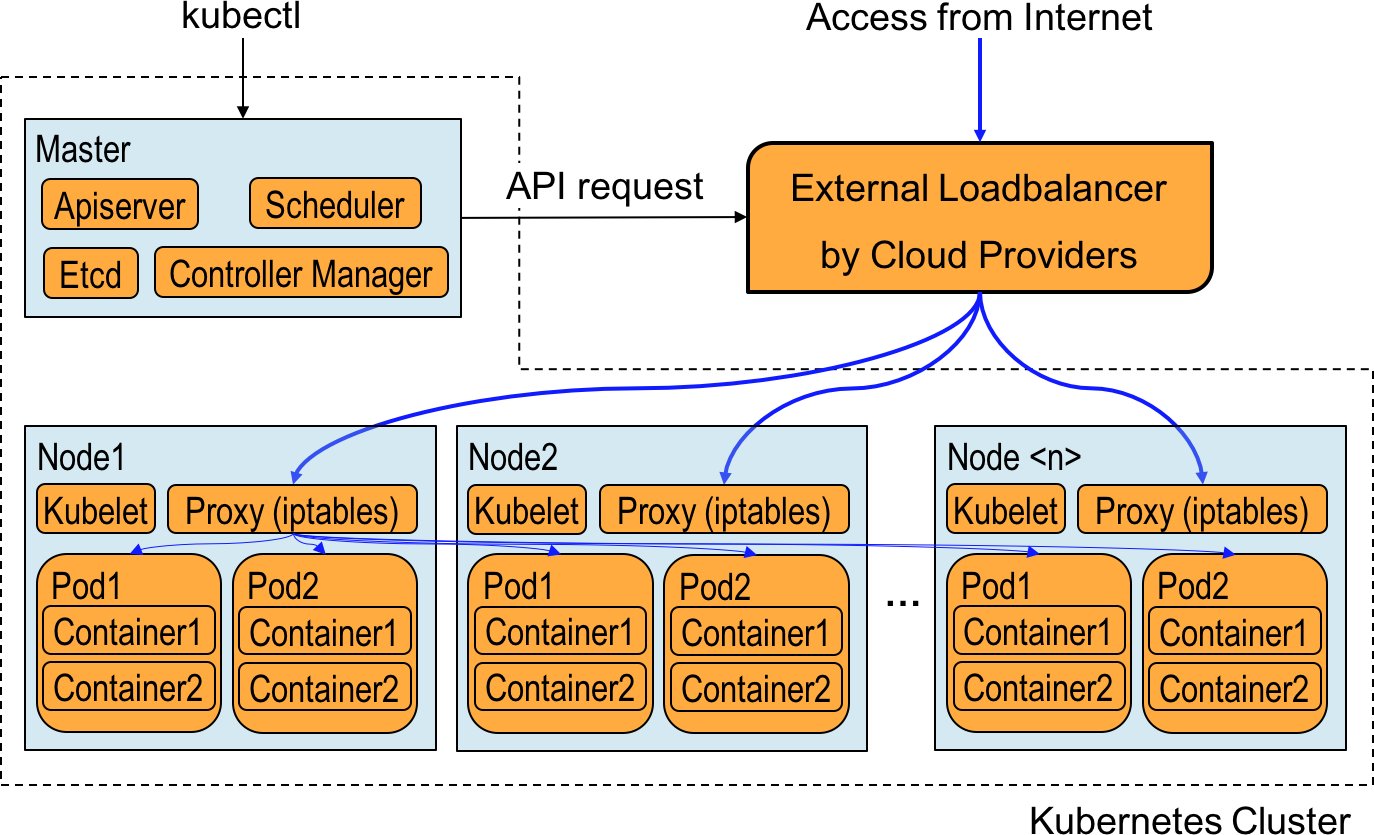
\includegraphics[width=0.8\columnwidth]{Figs/K8sConventional}
    \caption{Kubernetes in cloud infrastructures}
    \label{fig:K8sConventional}
  \end{subfigure}

  \par\bigskip
  \par\bigskip

  \begin{subfigure}[t]{\columnwidth}
    \centering
    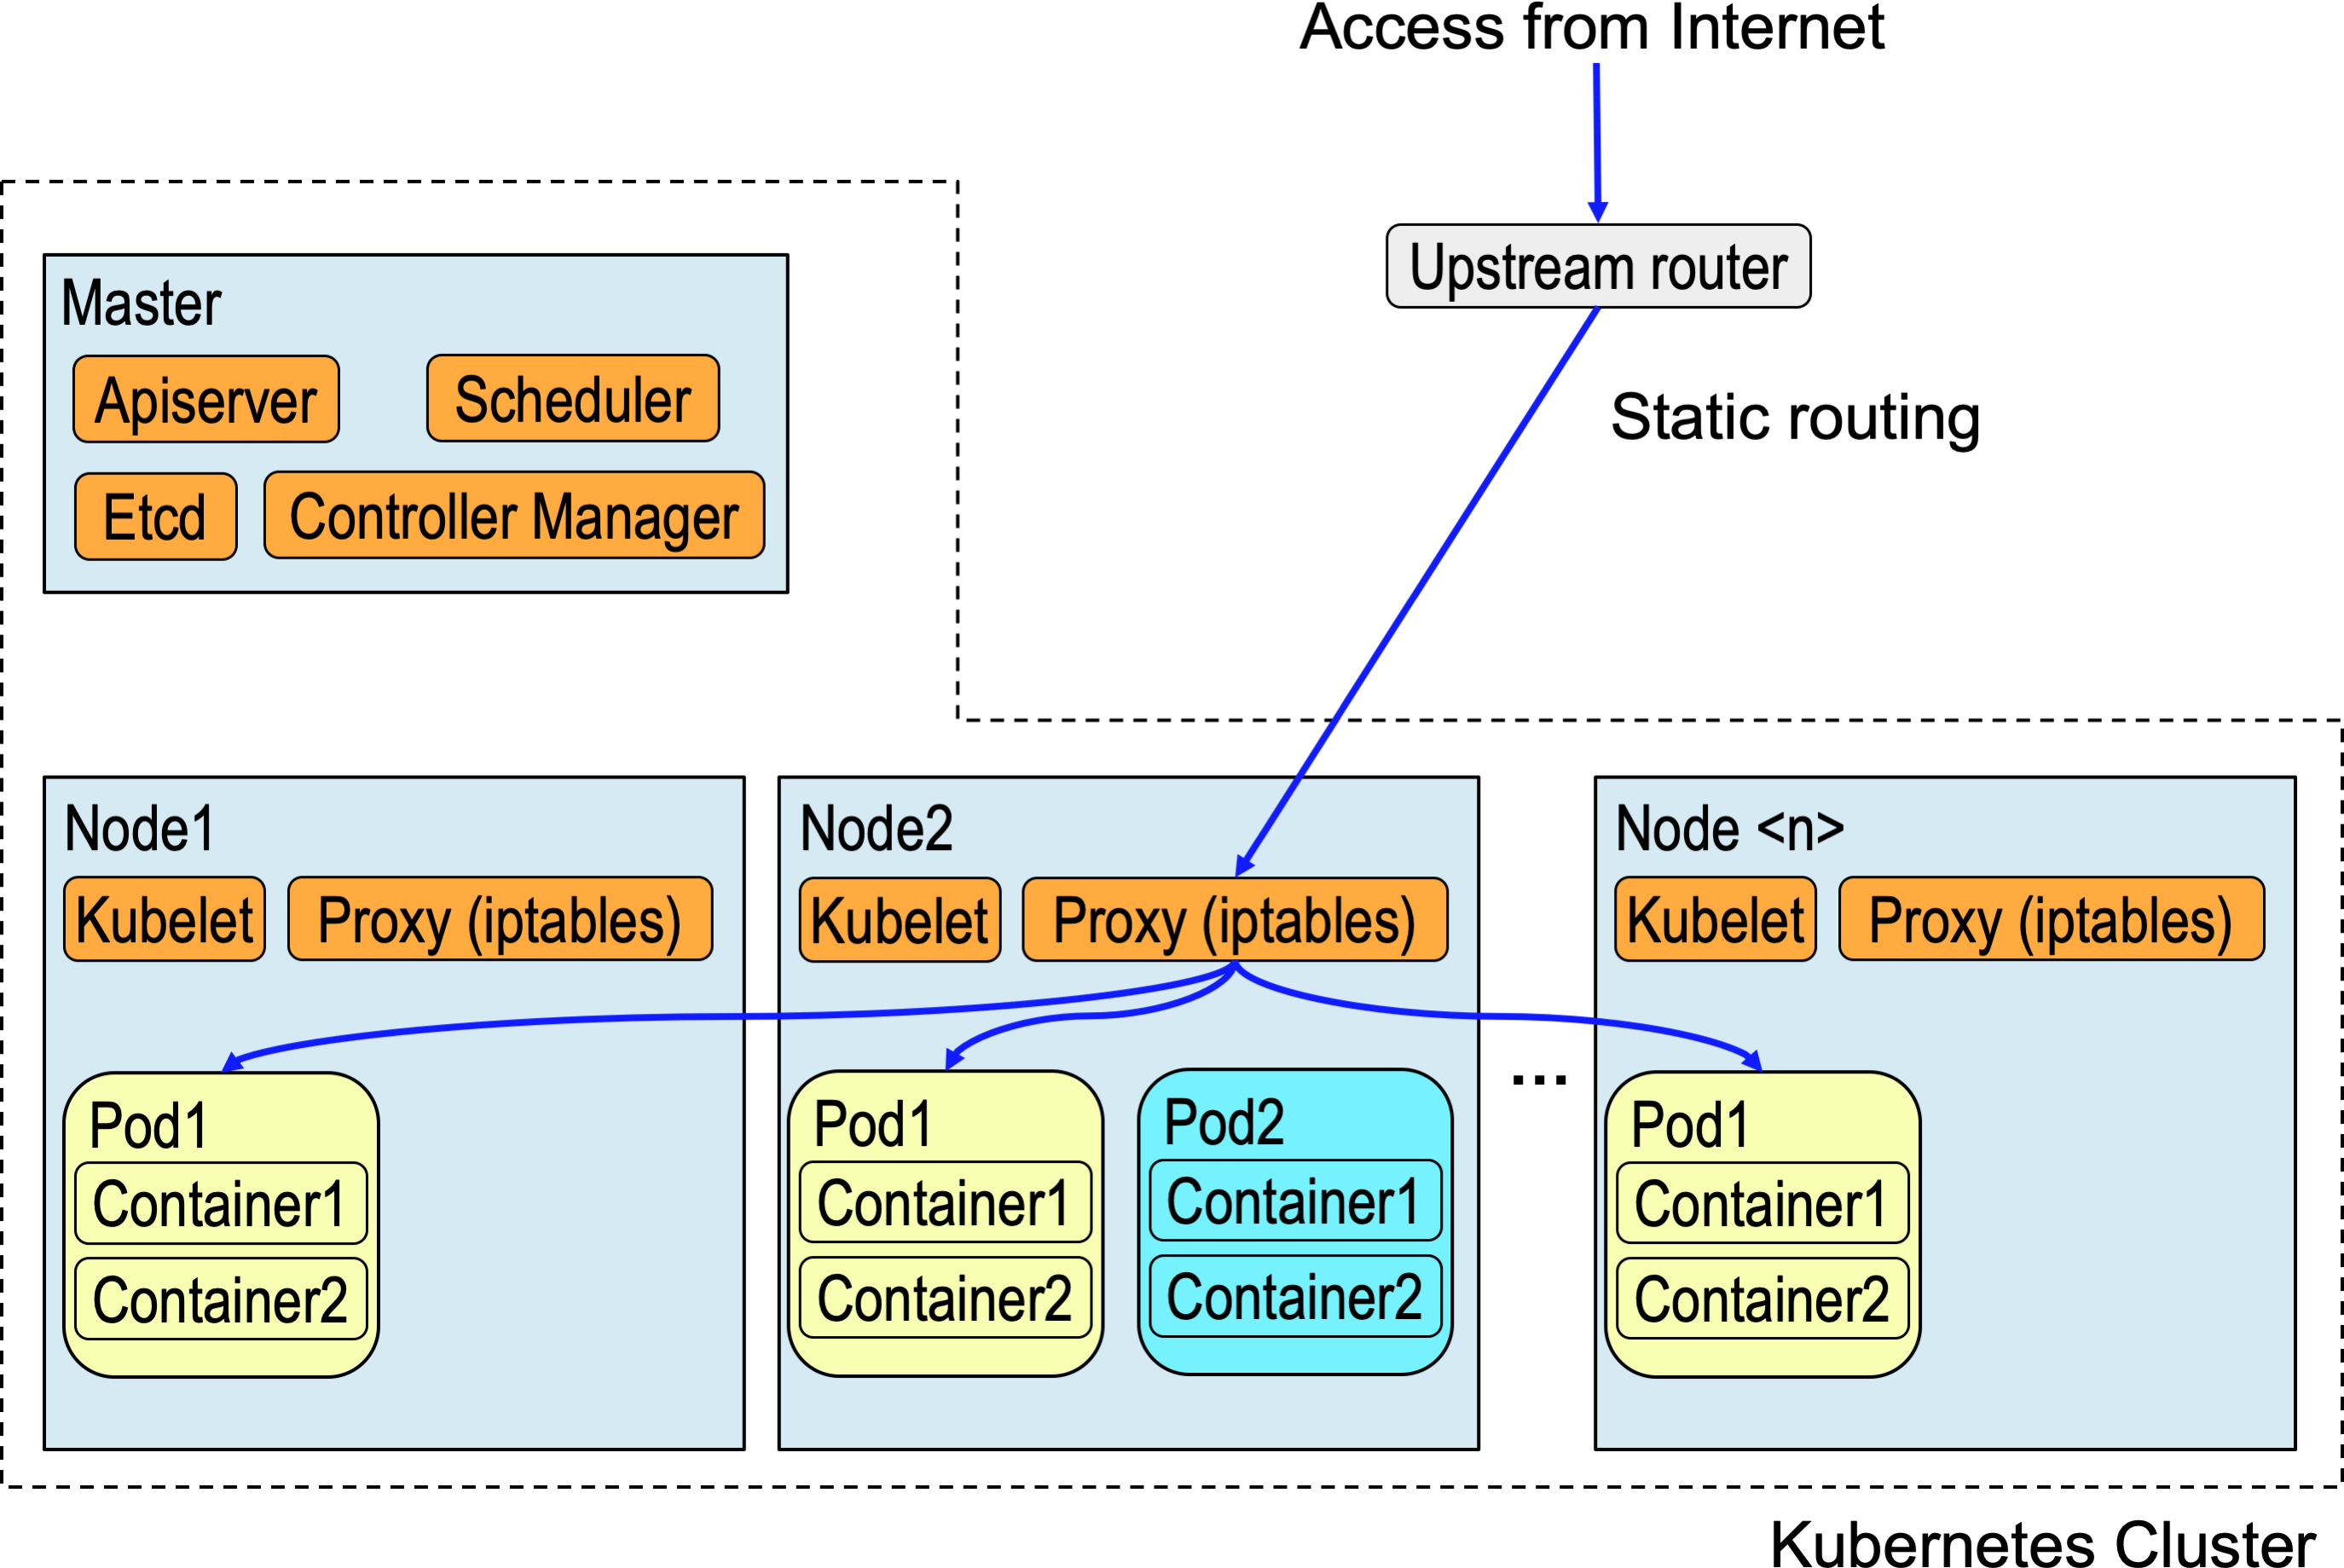
\includegraphics[width=0.8\columnwidth]{Figs/K8sConventional_bm}
    \caption{Kubernetes in on-premise data centers}
    \label{fig:K8sConventional_bm}
  \end{subfigure}

   \centering

  \begin{minipage}{1.0\columnwidth}
    \caption[Conventional architecture of Kubernetes clusters]
            {Conventional architecture of Kubernetes clusters in cloud infrastructure and on-premise data center.
%\small
(a) In supported infrastructures, e.g., major cloud providers, Kubernetes automatically set up the routes for ingress traffic with the help of the external load balancer.
The load balancer distributes ingress traffic to all of the existing nodes.
(b) In unsupported infrastructures, e.g., on-premise data centers, web application providers have to manually set up a route to one of the nodes.
Packets that reached any of the nodes will be distributed to appropriate pods by the iptables DNAT based internal load balancer.
            }
  \end{minipage}

\end{figure}

The problem of Kubernetes is its partial support for the ingress traffic routing.
Figure~\ref{fig:K8sConventional} shows an exemplified Kubernetes cluster.
When a service is created, the master schedules where to run {\em pods}, and kubelets on the nodes launch them accordingly.
At the same time, the master sends out requests to cloud provider's API endpoints, asking them to set up external cloud load balancers that distribute ingress traffic to every node in the Kubernetes cluster.
The proxy daemon on the nodes also setup iptables DNAT\cite{MartinA.Brown2017} rules. 
The Ingress traffic will then be evenly distributed by the cloud load balancer to all the existing nodes, 
after which it will be distributed again by the DNAT rules on the nodes to the designated {\em pods}. 
The returning packets follows the exact same route as the incoming ones.

This architecture has the followings problems: 
1) There must exist cloud load balancers whose APIs are supported by the Kubernetes daemons.
There are numerous load balancers which is not supported by the Kubernetes.
These include the bare metal load balancers for on-premise data centers.
2) Distributing the traffic twice, first on the external load balancers and second on each node, complicates the administration of packet routing. 
Imagine a situation in which the DNAT table on one of the nodes malfunctions.
In such a case, only occasional timeouts would be observed, and hence it would be very difficult to find out which node is malfunctioning.   
3) The ingress traffic is distributed to all the existing nodes in the Kubernetes cluster. 
Suppose there are 1,000 nodes and one of web applications only uses 10 nodes, it seems inefficient and rather complicated to distribute the ingress traffic to all the 1,000 nodes.

Regarding the first problem, if there is no load balancer that is supported by Kubernetes, users must manually set up the static route on the upstream router, every time they launch the web application clusters, as is shown in Figure~\ref{fig:K8sConventional_bm}.
The traffic will be routed to a node and then distributed by the DNAT rules on the node to the designated {\em pods}.
In cases where the upstream router is administered by a data center company, users must always negotiate with them about adding a route to their new application cluster.
This approach significantly lacks simplicity, and degrades the portability of container clusters.
Furthermore, a static route usually lacks redundancy and scalability.

In short, while Kubernetes is effective in major cloud providers, it fails to provide portability for container clusters in environments where there is no supported load balancer. 
And the routes incoming traffic follow are very complex and inefficient.
In order to address these problems, the author proposes a containerized software load balancer 
that is deployable in any environment even if there are no external load balancers.

\FloatBarrier

\subsection{Load balancer in container}\label{Load balancer in container}

The author proposes a load balancer architecture, where a cluster of load balancer containers is deployed as a part of web application cluster.
Figure~\ref{fig:K8sProposed} shows the proposed load balancer architecture for Kubernetes,
which has the following characteristics;
1) A cluster of load balancer containers is deployed as a part of web application cluster.
2) Each load balancer itself is run as a {\em pod} by Kubernetes.
3) Load balancing rules are dynamically updated based on the information about running {\em pods}, which is periodically populated by communicating with apiserver on the master.
4) There exist multiple load balancers for redundancy and scalability.
5) The routing table in the upstream router is updated dynamically using standard network protocol, BGP.

\begin{figure}[h]
  \begin{center}
  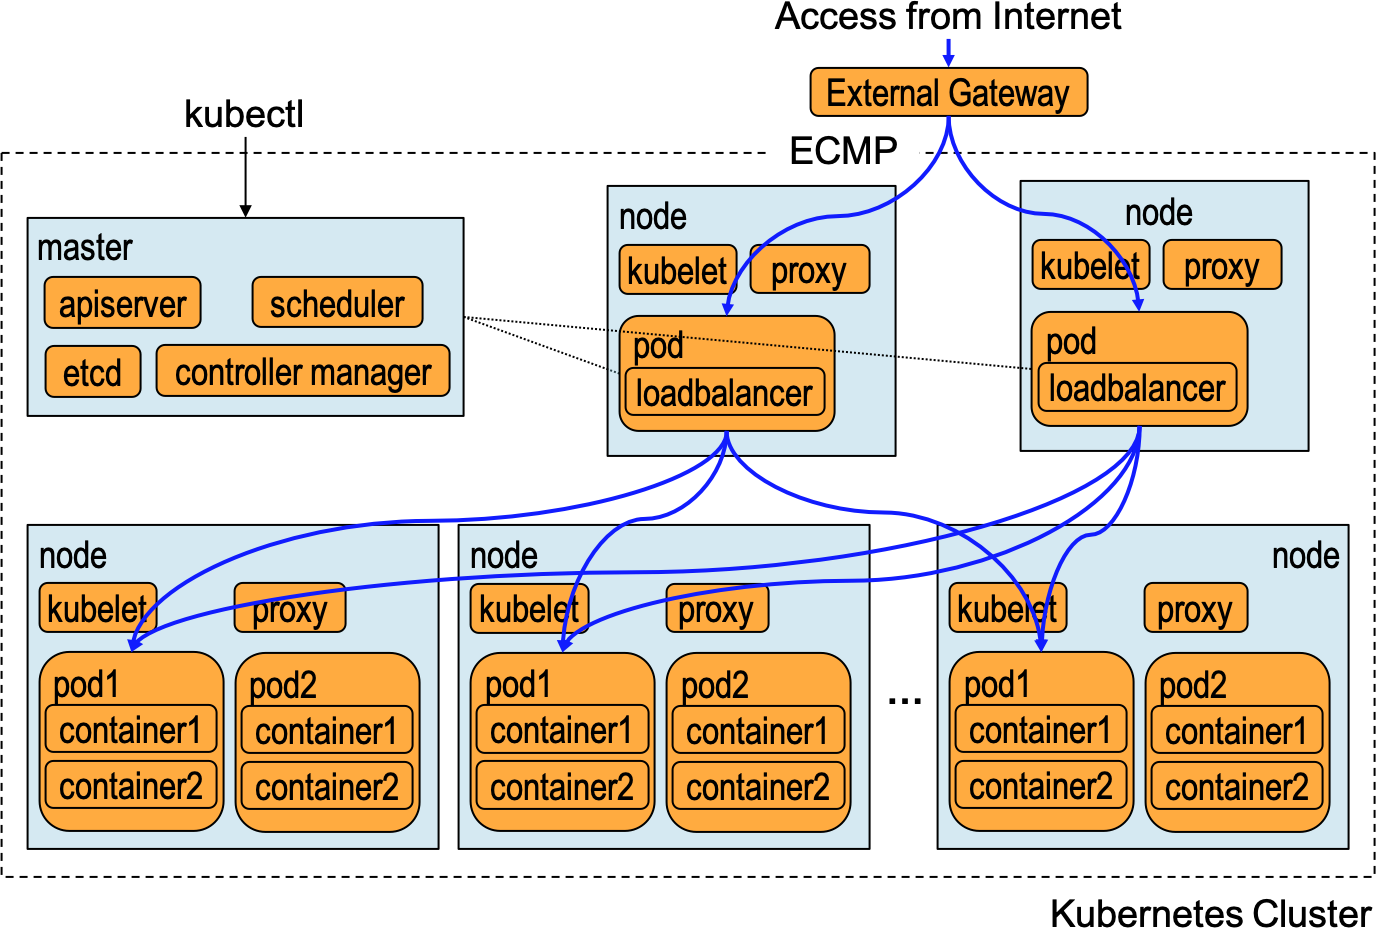
\includegraphics[width=0.8\columnwidth]{Figs/K8sProposed}
  \caption{Kubernetes cluster with proposed load balancer.}
  \label{fig:K8sProposed}
  \begin{minipage}{0.9\columnwidth}
  A cluster of load balancer containers is deployed as a part of web application cluster.
  Each load balancer itself is run as a {\em pod} in the Kubernetes cluster. 
  Load balancing rules are dynamically updated based on the information about running {\em pods}.
  There exist multiple load balancers for redundancy and scalability.
  The routing table in the upstream router is updated dynamically using standard network protocol, BGP.
  \end{minipage}
  \end{center}
\end{figure}

The proposed load balancer can resolve the conventional architecture problems.
Since the load balancer itself is containerized, the load balancer can run in any environment including on-premise data centers,
even without external load balancers that is supported by Kubernetes.
The incoming traffic is directly distributed to designated {\em pods} by the load balancer.
It makes the administration, e.g. finding malfunctions, easier.
Since the proposed load balancers are deployed as a part of web application cluster and the routes to the load balancers are set up automatically through BGP, users do not need to manually set up a static route to a load balancer.

Furthermore, the proposed load balancer has other benefits.
Since a software load balancer in a container can run on any Linux system, it can share the server pool with web containers.
Users can utilize existing servers rather than buying dedicated hardware.

Because a cluster of load balancer containers is controlled by Kubernetes, it becomes redundant and scalable.
Kubernetes always tries to maintain the number of load balancer containers as same as the number specified by the user.
If a single container fails, Kubernetes schedule and launch another one on a different node, which provides the resilience to failures.
When there is a huge spike in the traffic, user can quickly scale the size of the cluster depending on the demand.

The routes to the load balancers are automatically updated through the standard protocol, BGP.
Therefore users do not need to manually add the route every time new load balancer container is launched, as is the case in the conventional architecture.

\FloatBarrier

\subsection{Redundancy with ECMP}\label{Redundancy with ECMP}

\begin{figure}[tb]
  \centering
  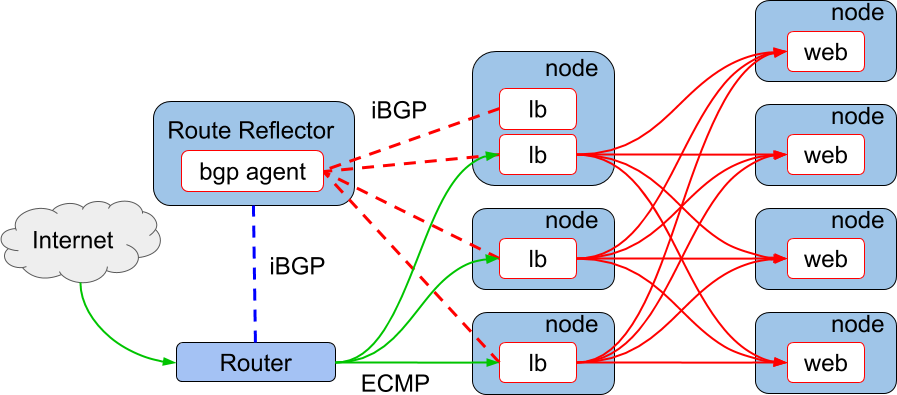
\includegraphics[width=0.8\columnwidth]{Figs/ecmp.png}
\caption{The proposed architecture of load balancer redundancy with ECMP}

\vspace{1mm}

\begin{minipage}{0.9\columnwidth}
   The traffic from the internet is distributed by the upstream router to multiple of load balancer(lb) pods using hash-based ECMP(the solid green line), after which distributed by the lb pods to web pods using Linux kernel's ipvs(the solid red line).
  The route toward a service IP is advertised to the route reflector(the dotted red line), after which advertised to the upstream router(the blue dotted line) using iBGP.
%  For the green lines, a service IP address is used. The red lines use the IP addresses of the overlay network. The blue line uses the IP addresses of the node network.
\end{minipage}

\label{fig:ecmp}
\end{figure}

While containerizing ipvs makes it runnable in any environment, it is essential to discuss how to route the ingress traffic to the ipvs container.
The author proposes redundant architecture using ECMP with BGP for proposed load balancer containers.

Fig.~\ref{fig:ecmp} shows a schematic diagram to explain redundancy architecture with ECMP for the proposed load balancer.
%
The ECMP is a functionality a router supports, where the router has multiple next hops with equal priority(cost) to a destination.
And the router generally distributes the traffic to the multiple next hops depending on the hash of five-tuples(source IP, destination IP, source port, destination port, protocol) of the flow.
The multiple next hops and their cost are often populated using the BGP protocol.
%
The notable benefit of the ECMP setup is its scalability.
All the load balancers that claims as the next hop is active, i.e., all of them are utilized to increase the performance level.
Since the traffic from the internet is distributed by the upstream router, the overall throughput is, after all, limited by performance levels of the router.
However, in practice, there are a lot of cases where this architecture is beneficial.
For example, if a software load balancer is capable of handling 1 Gbps equivalent of traffic and the upstream router is capable of handling 10 Gbps, it still is worthwhile launching 10 of the software load balancer containers to fill up maximum throughput of the upstream router.

%
In the proposed redundant architecture, there exists a node with the knowledge of the overlay network as a route reflector.
A route reflector is a network component for BGP to reduce the number of peerings by aggregating the routing information\cite{rfc4456}.
In the proposed architecture the author uses it as a delegater for load balancer containers towards the upstream router.

The route reflector exists for a practical reason, i.e, to deal with the complexity due to the overlay network.
Since the upstream router normally has no knowledge of the overlay network and IP addresses used inside the Kubernetes clusters, a container must rely on SNAT on the node to communicate with the router.
The SNAT caused a problem when the author tried a set up without the route reflector, to co-host multiple load balancer containers for different services on a single node.
Because of the SNAT, the source IP addresses of multiple connections were translated into a single IP address possessed by the node.
The BGP agent on the router was confused by these connections and could not properly set up ECMP routes for separate services.
This was due to the fact that the BGP agent used in the experiment used only the source IP address of the connection to distinguish the BGP peer.

In addition to that, the route reflector brings another benefit.
The upstream router does not need to accept BGP sessions from containers with random IP addresses, but only from the route reflector with well known fixed IP address.
This is preferable in terms of security especially when a different organization administers the upstream router.

By using the route reflector, we can have the following benefits.
1) Each node can accommodate multiple load balancer containers. This was not possible when we tried to directly connect load balancers and the router through SNAT.
2) The router does not need to allow peering connections from random IP addresses that may be used by load balancer containers. Now, the router only need to have the reflector information in the BGP peer definition.

Since a standard Linux system is used for the route reflector, it can be configured as we like;
a) It can be configured to belong to the overlay network so that multiple BGP sessions from containers on a single node can be properly distinguished.
b) One can select a BGP agent that supports dynamic neighbor (or dynamic peer), where he only needs to define the IP range as a peer group and does away with specifying every possible IP that load balancers may use.
Although not shown in the Fig.~\ref{fig:ecmp}, it is possible to have another route reflector for redundancy purpose.

\FloatBarrier


